\graphicspath{{images/chapter2/}}

\chapter{Pose Estimation Model Selection and Baseline}
\label{chap:baseline}

The goal is to improve pose estimation on art collections.
For this effort, two methods will be investigated: 
First, the input to existing models will be transformed from artworks to photographs.
Second, the models will be retrained on an COCO dataset which is augmented with synthetic COCO images.
In the previous section, a style transfer model was trained for this, and now, a proper baseline needs to be established to compare to the results of the experiments.
This chapter will determine that baseline.
For this, two pose estimation algorithms will be explored.
The motivation for the choices of the algorithms will be explained in full detail.
The focus will be on quality instead of speed.
The precision of pre-trained pose estimation models will be measured on the COCO dataset to establish a ground truth.
Afterwards, the pre-trained models will be validated on the Human-Art dataset and the stylized COCO dataset.
The results of that will give an indication of how well pose estimation works on art collections and where there's room for improvement.
\\

There are several considerations to be made when choosing the right model.
The focus will mainly be on methods that have code readily available.
The model must also be compatible with the preferred dataset.
Pose estimation has several datasets with different amounts of keypoints, bounding boxes or other metadata.
The most popular dataset and supported by most models will be used, which is the COCO dataset.
The main aspect of the problem is quality and speed.
When setting up a database for querying, there needs to be qualitative results to search through.
The search itself should be fast, but this is not the subject of this thesis.
At the same time, there should be a wide variation in architectures as explained previously (Chapter \ref{chap:style_transfer}).
All these criteria are considered in the next sections as well as those uniquely for each section.

\section{Baseline Pose Estimation}

\subsection{Choice of Model}
\label{sec:baseline_choice_pose_estimation}
Here again, quality is the most important criteria for performance.
The current state-or-the-art is ViTPose \cite{xu2023}.
The model is based on vision transformers.
This makes it an obvious first choice.
An overwhelming amount of models both in top-down as well as bottom-up architectures use HRNet \cite{Sun2019} with the only difference being in pre-processing \cite{Zhang2019, Huang2019} or post-processing \cite{Cheng2019, Geng2021}.
Since VitPose is a top-down architecture and to keep a variety of architectures, a bottom-up version of HRNet is selected.
The best model in this family is SWAHR according to Chen et al. \cite{chen2022}.
Other architectures were looked at, like KAPAO \cite{William2021}, which uses a single-stage architecture, but these were not performant enough to be considered.

\subsection{Training}
\label{sec:baseline_training_pose_estimation}
For the sake of learning the different algorithms, the training methods were reverse engineered
So, it was deemed appropriate to train the chosen models from scratch, so there's a plain network trained with the new setup for comparison.
All training was done using the default parameters.

\section{Pose Estimation after Applying Style Transfer to the COCO Dataset}
\label{sec:baseline_coco_style_transfer}
Due to time constraints, the evaluation is only done on a subset of the COCO dataset.
This set was created by randomly sampling 1000 images.
The first baseline will establish how well the pre-trained models perform on a stylized COCO dataset.
The evaluated pose estimators will be SWAHR and ViTPose, and each will use the trained weights mentioned in section \ref{sec:baseline_training_pose_estimation}.
Since ViTPose is a top-down architecture, it will use the ground truth bounding box to extract the persons.
They will both be tested on a styled version of the COCO dataset by CycleGAN and AdaIN.
CycleGAN wil be applied for the 3 styles it was trained on; baroque, impressionism and renaissance.
AdaIN uses the pre-trained model and uses 3 images of each of the previous styles to use as style image.
The images were selected to best represent the style while also varying the content as shown in Figure \ref{fig:baseline_style_images_adain_evaluation}.
Each model uses the default parameters and at no time was the input image resized or otherwise distorted.
This comes to a total of 24 combinations that will be assessed.

\begin{figure}[h]
    \centering
	\subcaptionbox{Baroque style images}[\textwidth]{
		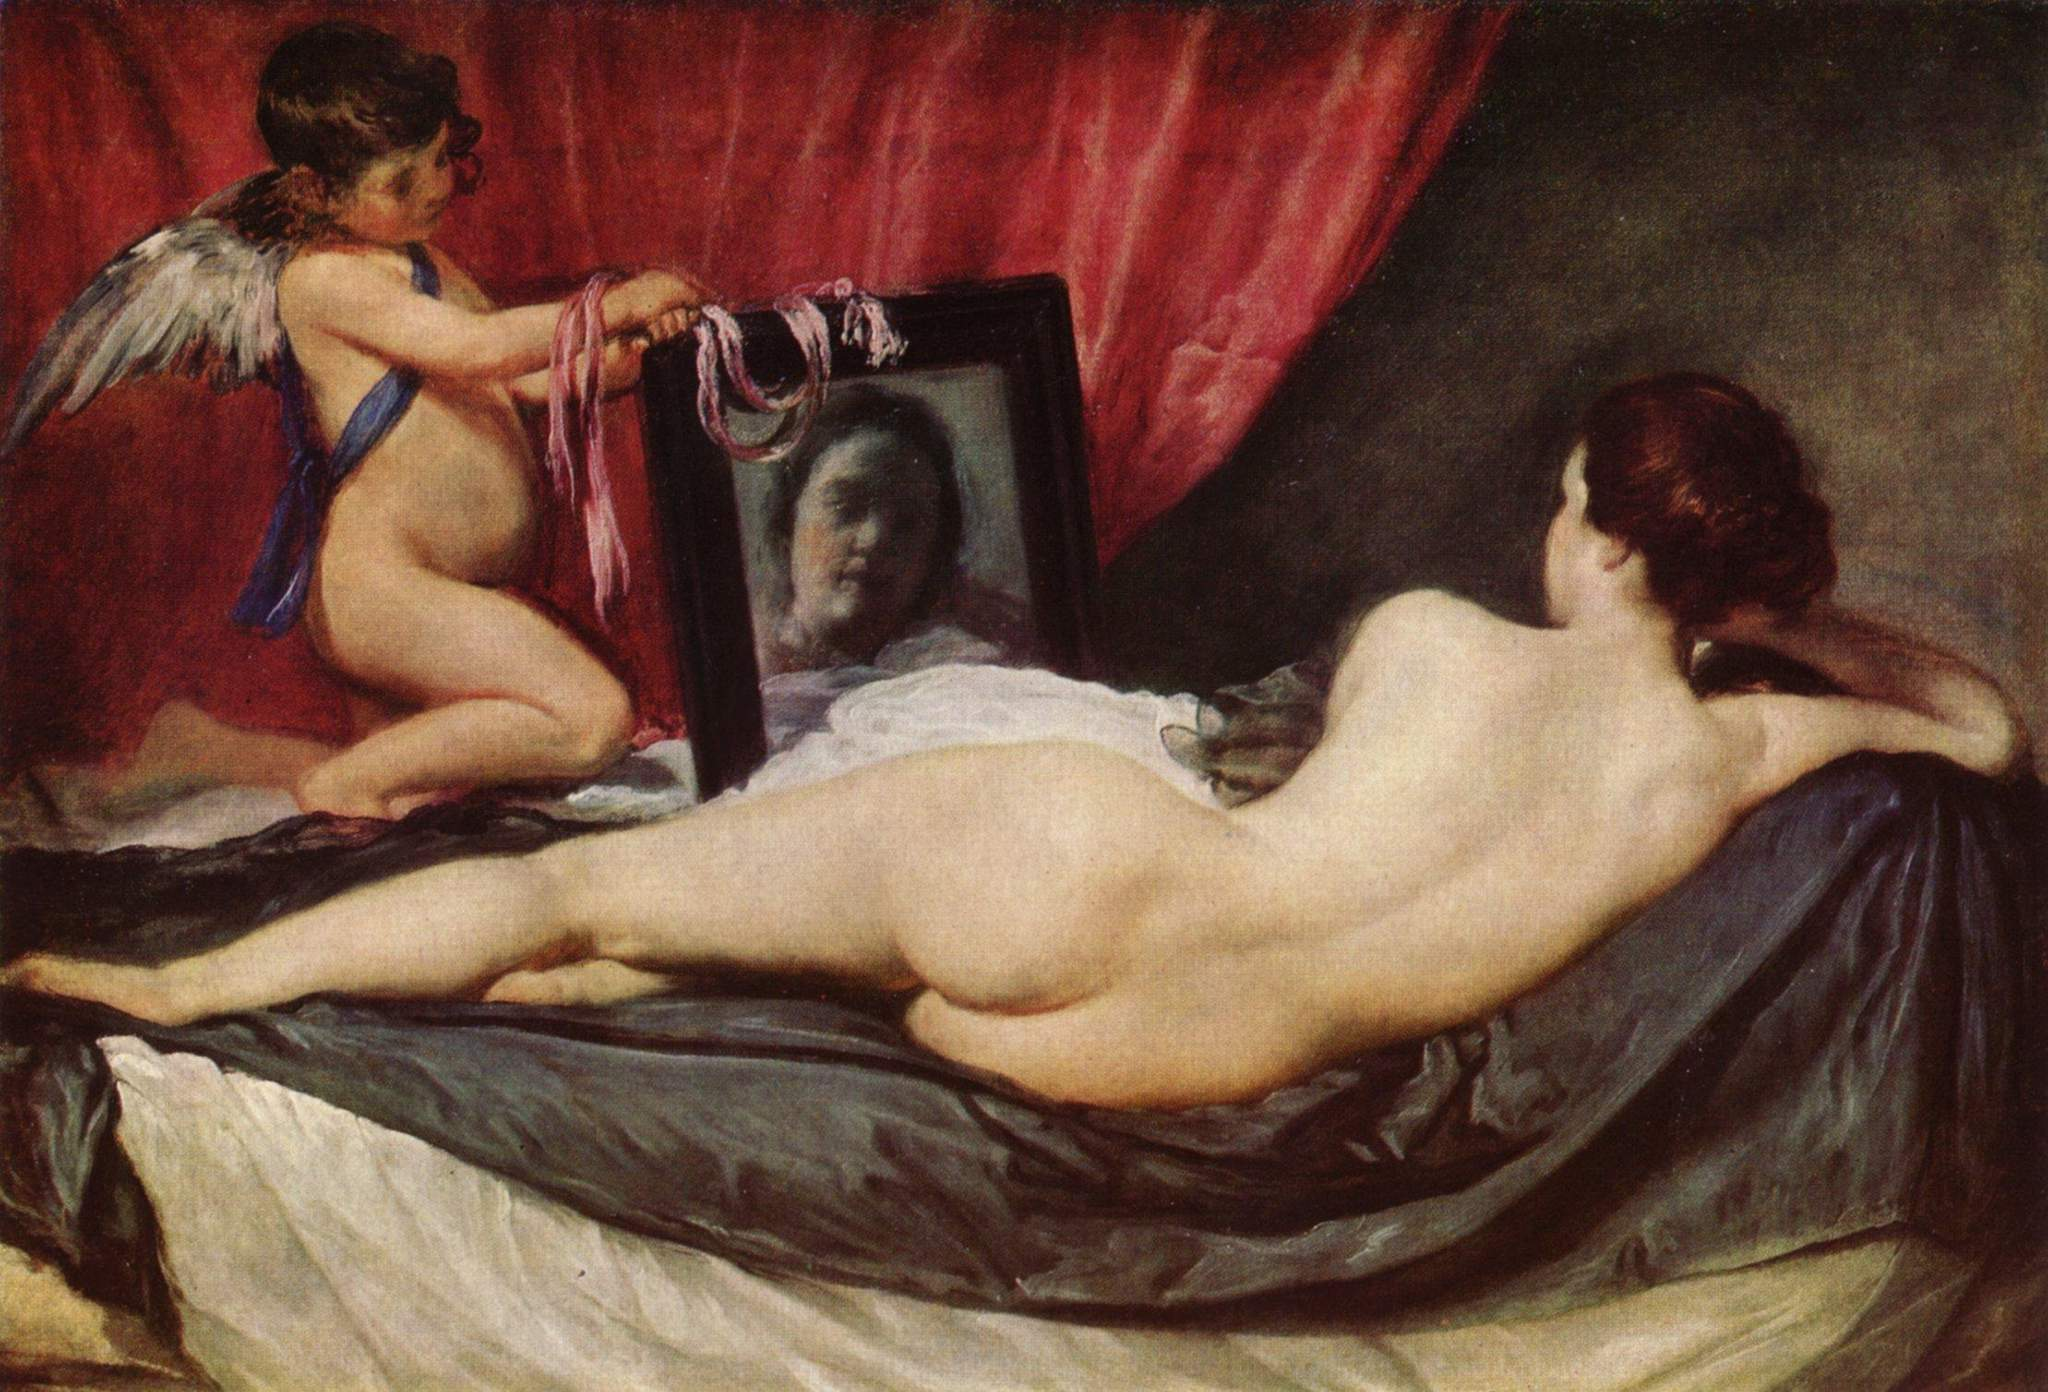
\includegraphics[height=1.25in]{22_22_diego-velazquez_the-rokeby-venus-1648}
		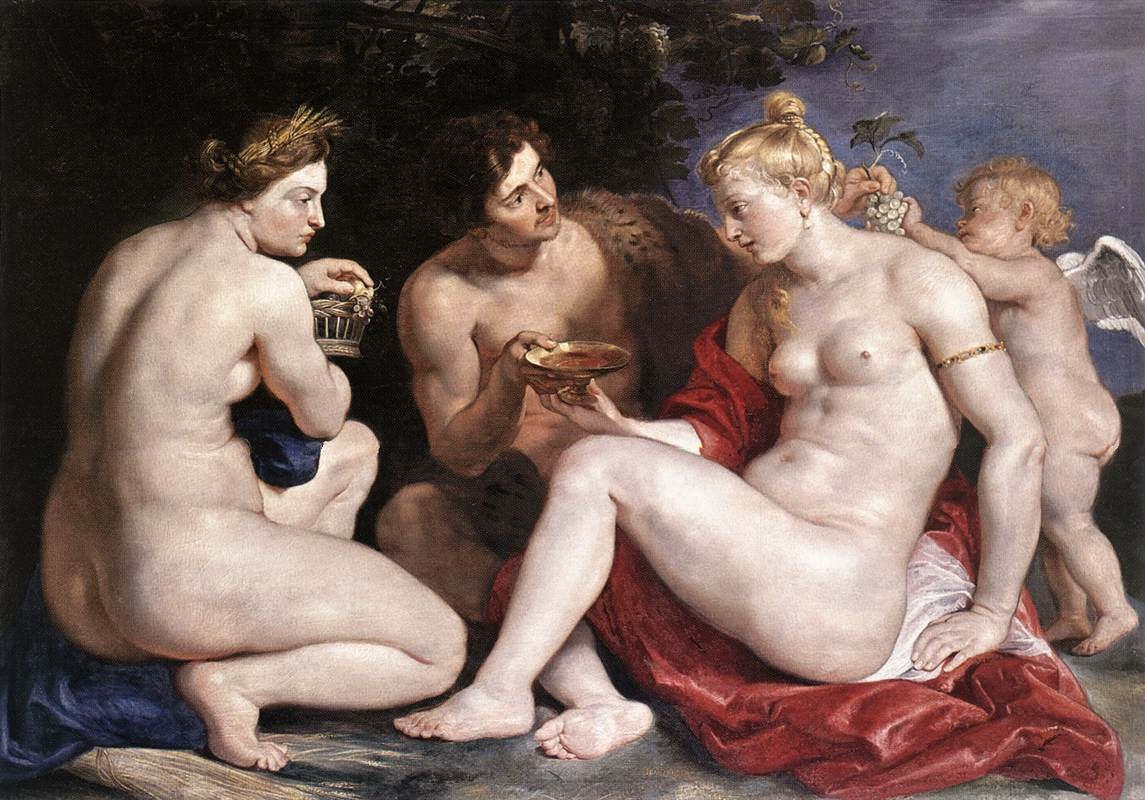
\includegraphics[height=1.25in]{100_1_peter-paul-rubens_venus-cupid-bacchus-and-ceres-1613}
		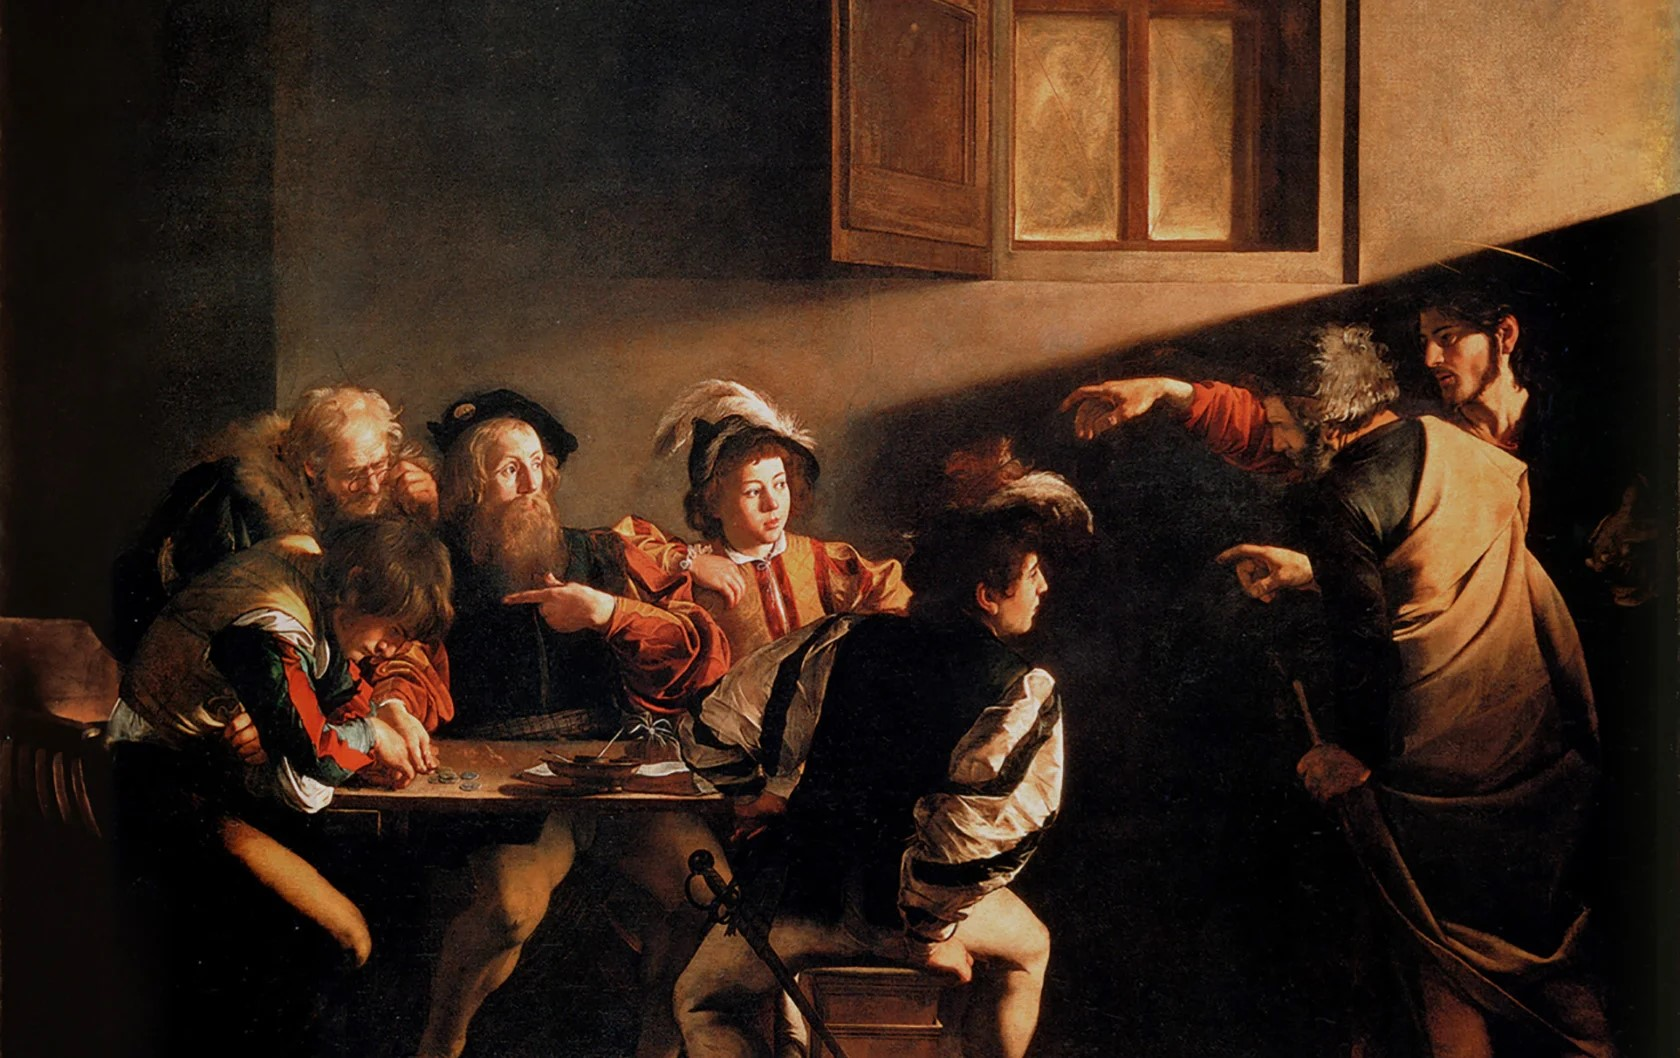
\includegraphics[height=1.25in]{caravaggio_the-calling-of-saint-matthew}
	}
	\subcaptionbox{Renaissance style images}[\textwidth]{
        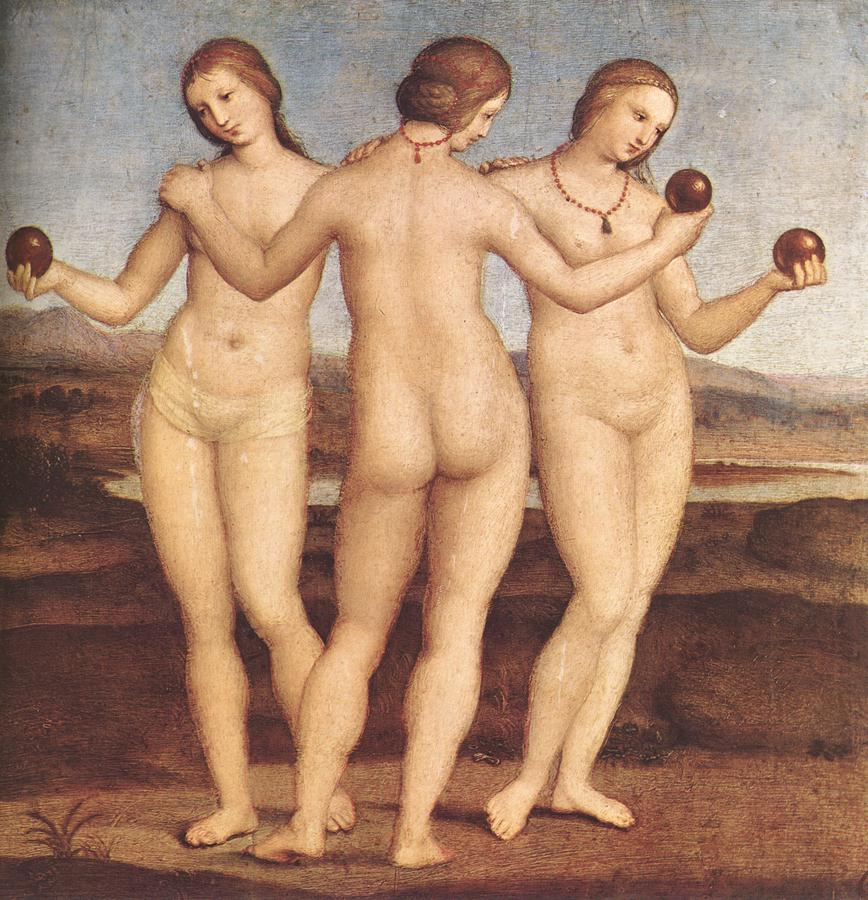
\includegraphics[height=1.25in]{26_4_raphael_the-three-graces-1505}
        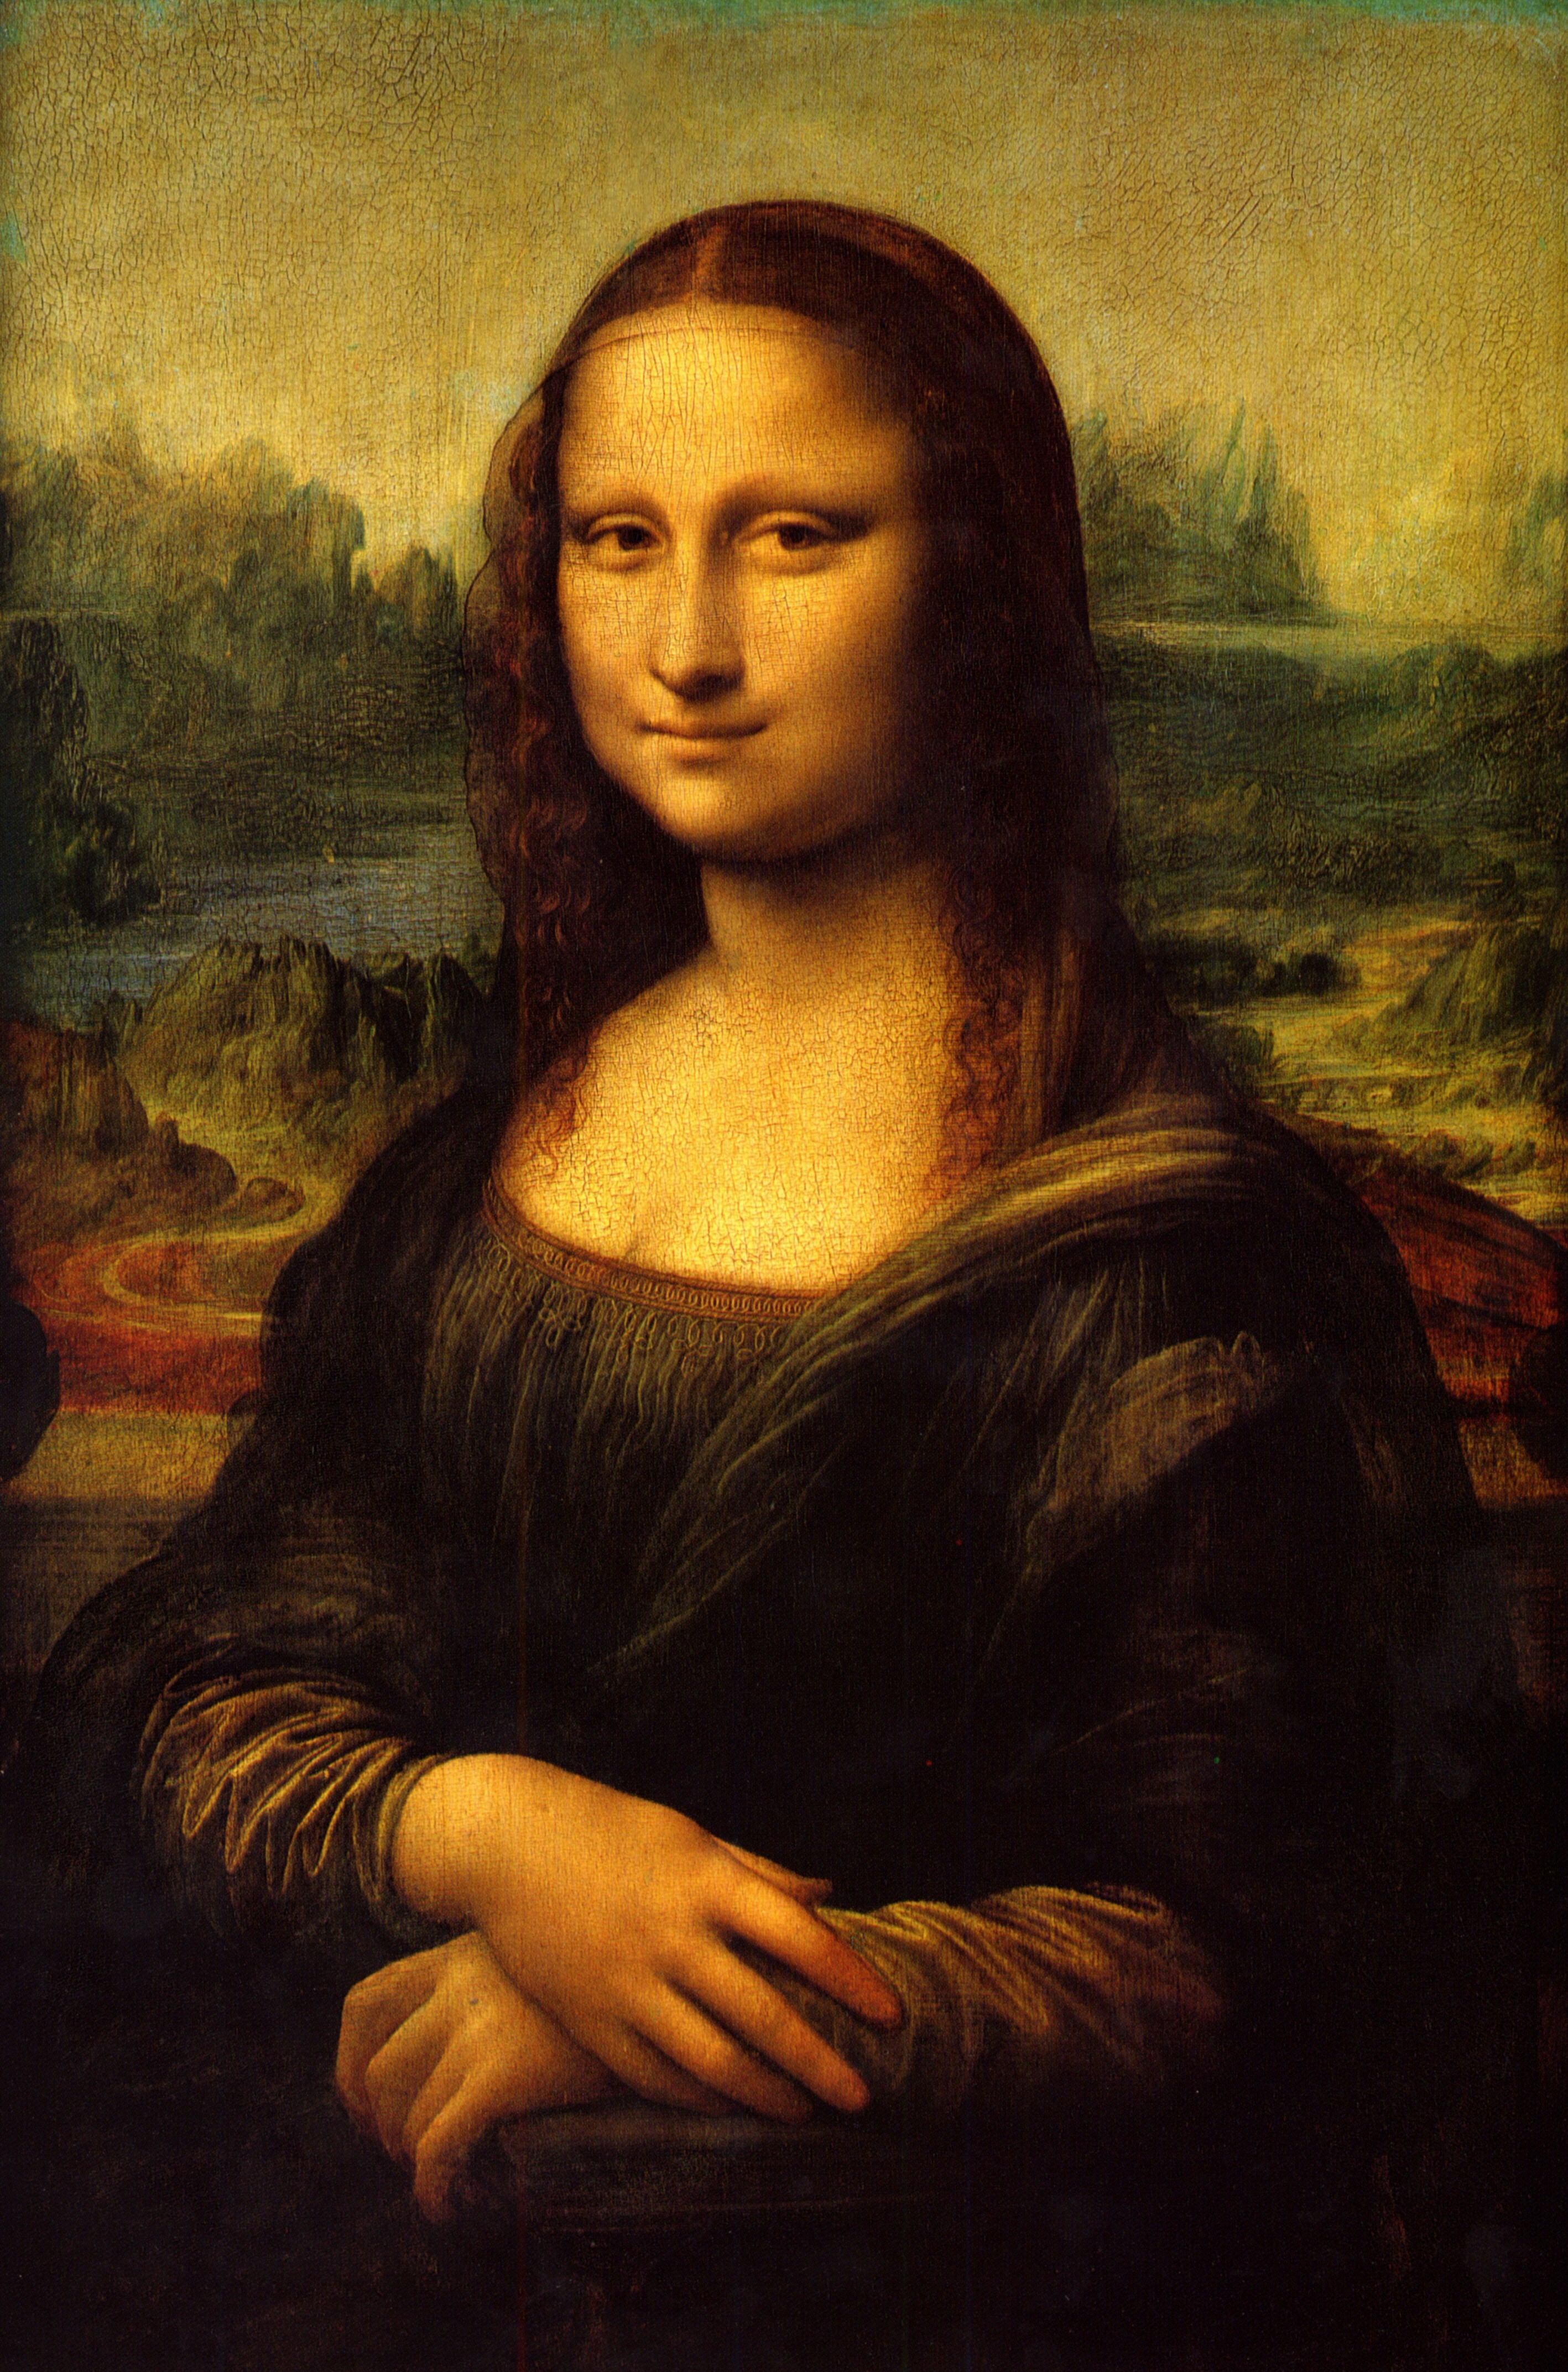
\includegraphics[height=1.25in]{15_11_leonardo-da-vinci_mona-lisa}
        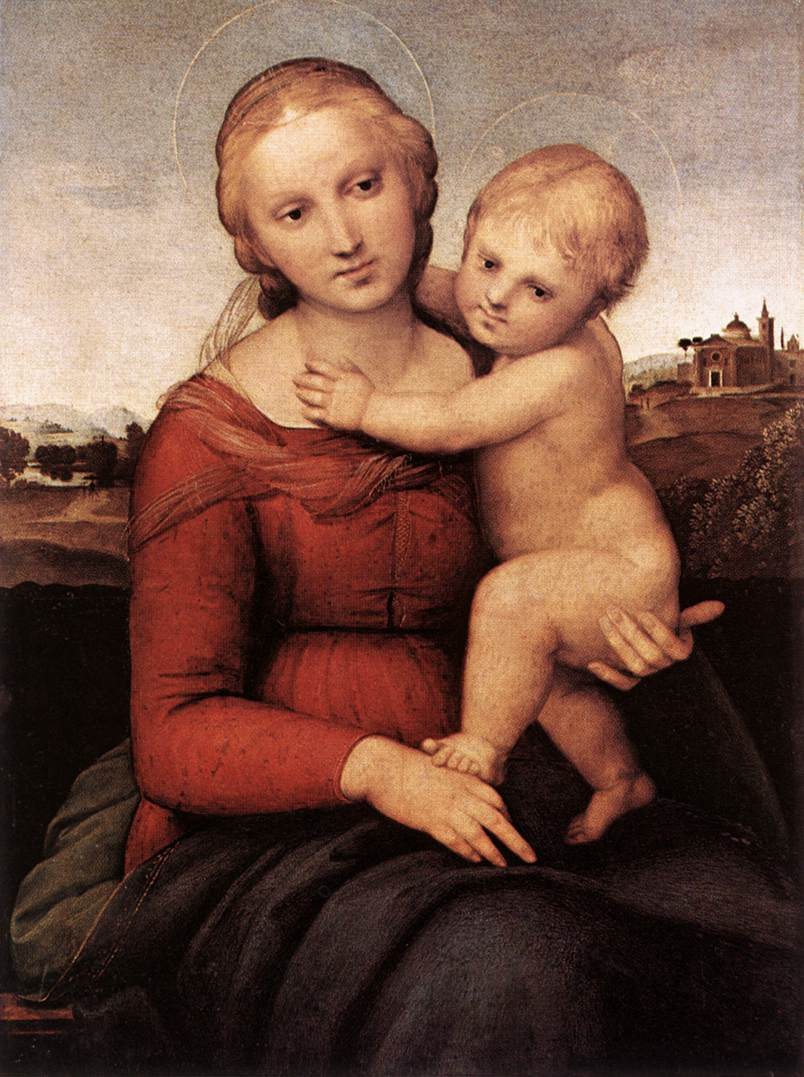
\includegraphics[height=1.25in]{26_5_raphael_madonna-and-child-1505}
	}
	\subcaptionbox{Impressionism style images}[\textwidth]{
        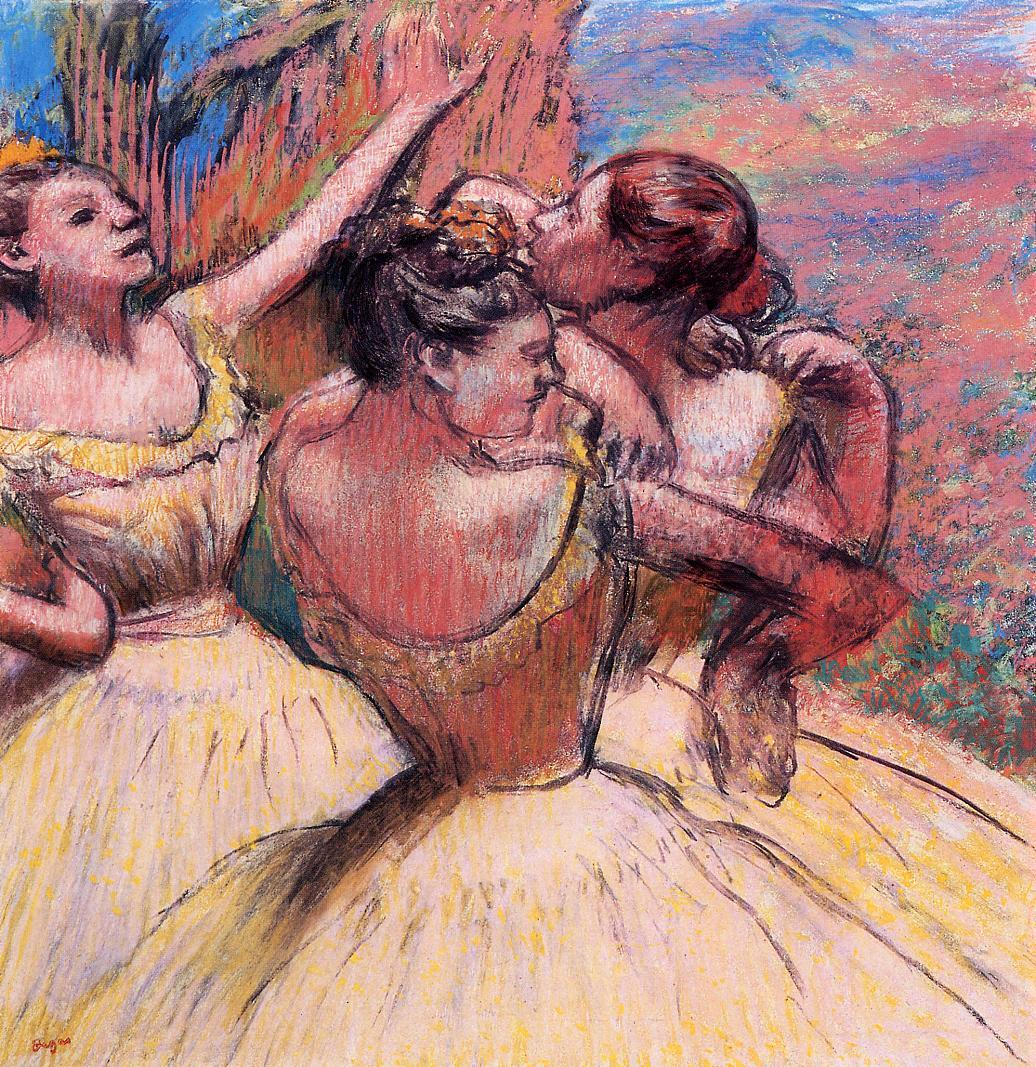
\includegraphics[height=1.25in]{22_91_edgar-degas_three-dancers}
        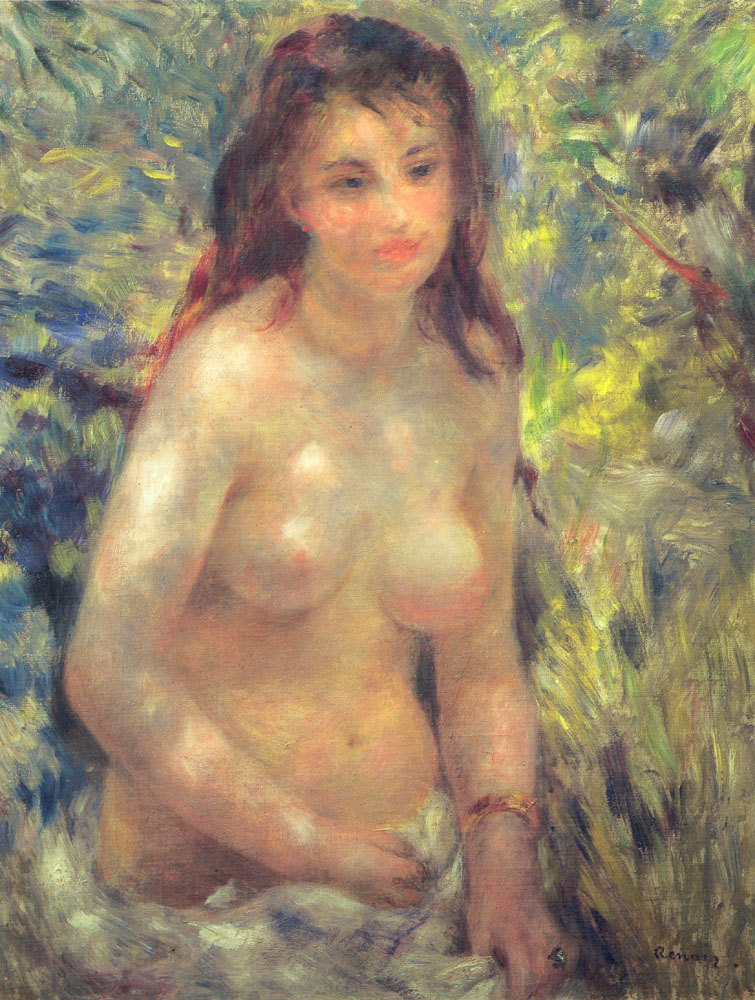
\includegraphics[height=1.25in]{26_21_pierre-auguste-renoir_study-torso-sunlight-effect}
        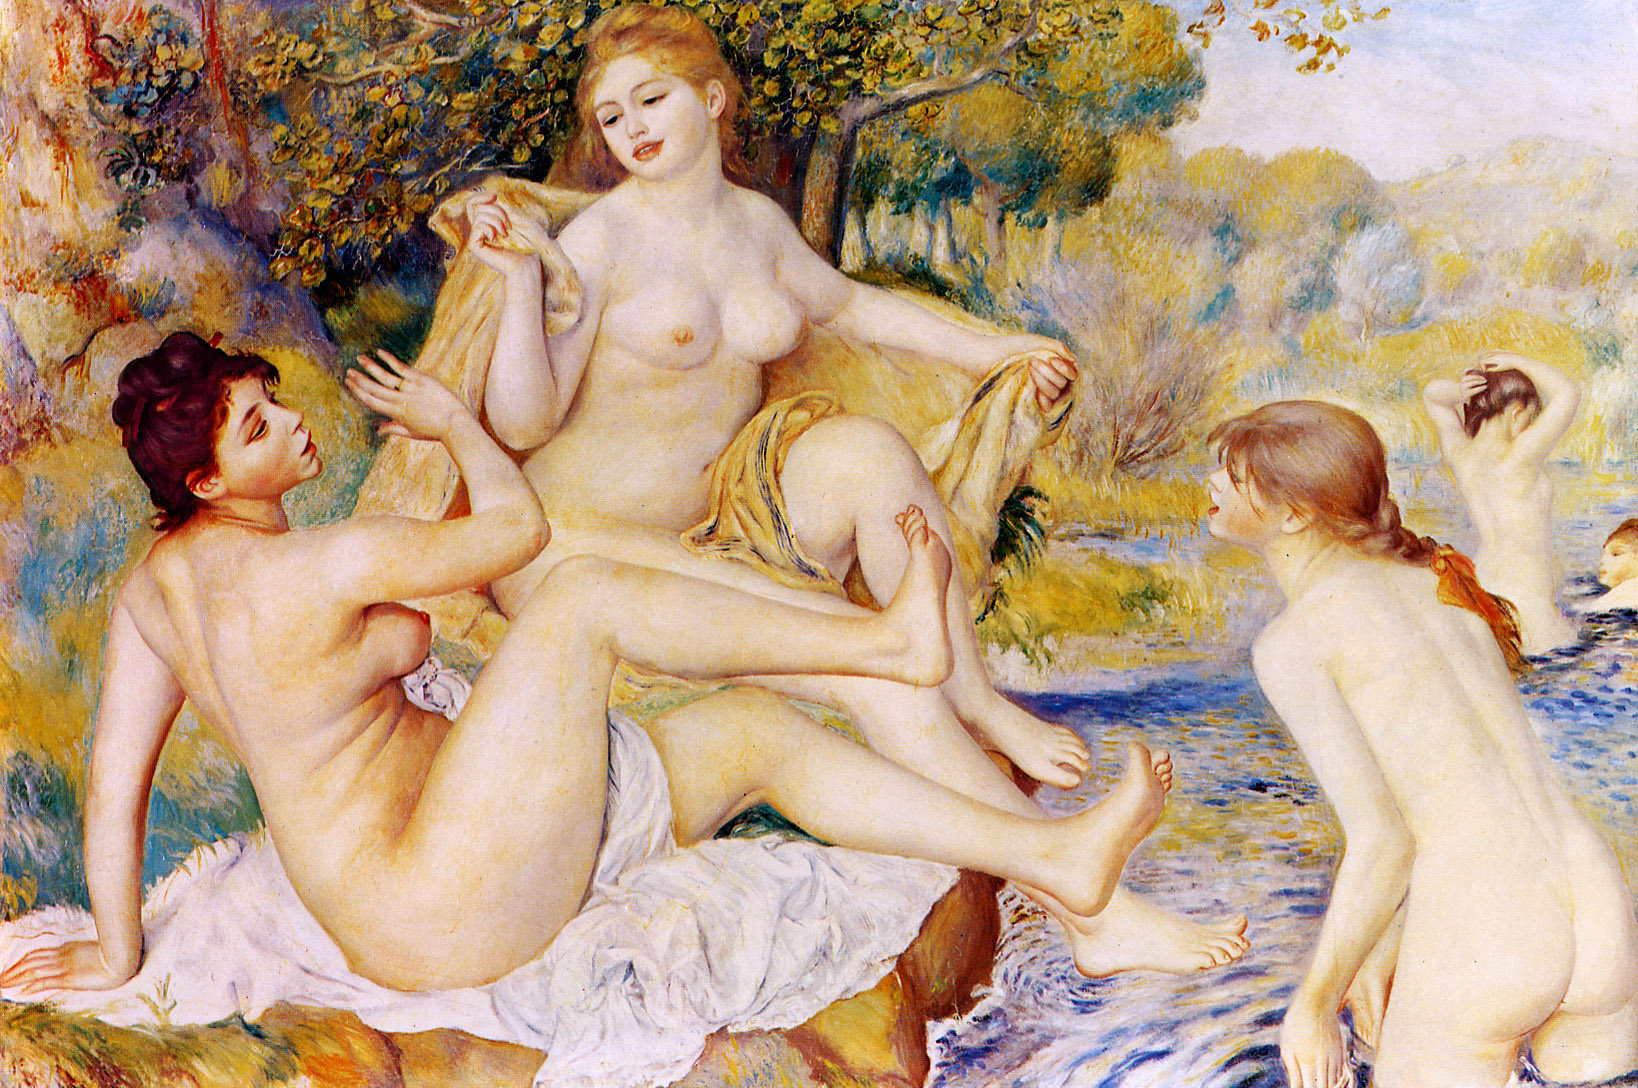
\includegraphics[height=1.25in]{99_1_pierre-auguste-renoir_the-large-bathers-1887}
	}
	\caption{
        The style images used for AdaIN during evaluation.
    }
    \label{fig:baseline_style_images_adain_evaluation}
\end{figure}

\subsection{Results}
\label{sec:baseline_results_coco_style_transfer}
From the available metrics the only ones that were useful for these measurements were the Average Precision/Recall.
They're implemented as part of the COCO dataset and work with any dataset that's compatible with the COCO format.
Of the other metrics, \gls{PCP} is unusable because it only applies to networks that detect the limbs as boxes instead of keypoints.
The chosen pose estimation networks only work with keypoints.
\gls{PCK} looked like it could be useable. However, PCKh needs a head bounding box, which is only available for the MPII dataset.
While all the implementations only work with top-down architectures.
They each asserts that the length of predicted persons should be the same as that of the ground truth.
In a bottom-up architecture, it is possible to find more or less persons.
The results shown in Table \ref{tab:baseline_pose_estimation_after_style_transfer} are the average of different evaluations, and it becomes immediately evident that this method is not going to work.
As seen in Figure \ref{fig:baseline_pose_estimation_evalutaion}, SWAHR is completely lost and can't find any good keypoints while ViTPose, having a high recall, still found some of the poses. 

\begin{figure}
    \centering
	\subcaptionbox{SWAHR}[\textwidth]{
		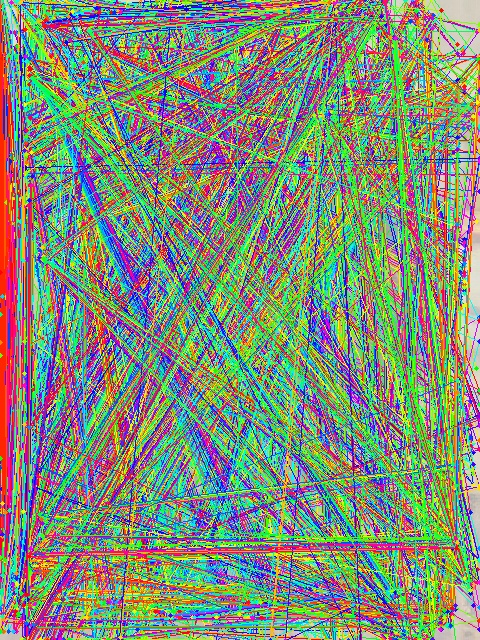
\includegraphics[height=1.75in]{swahr_7088}
		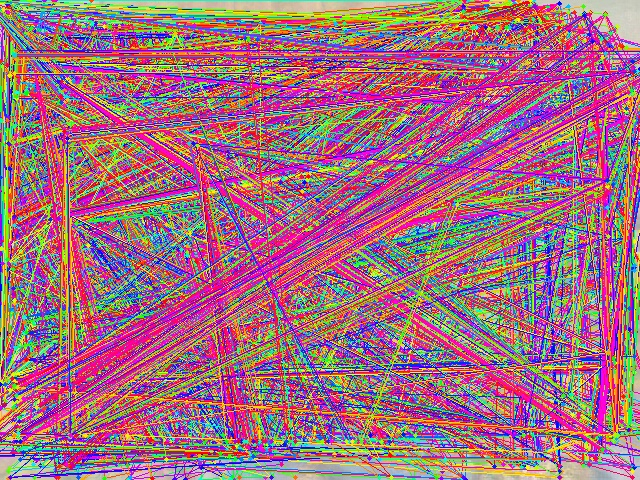
\includegraphics[height=1.75in]{swahr_91500}
		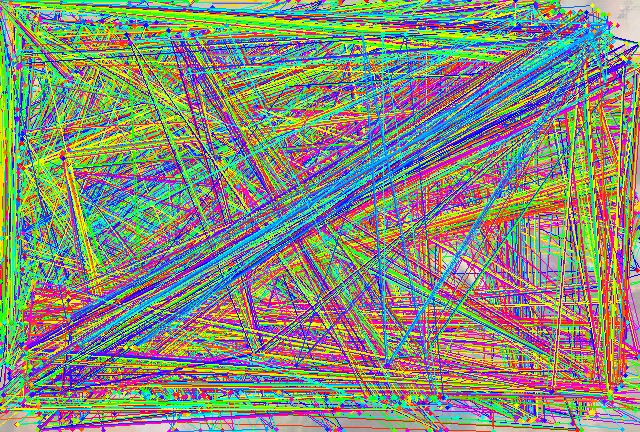
\includegraphics[height=1.75in]{swahr_259640}
    }
    \subcaptionbox{ViTPose}[\textwidth]{
		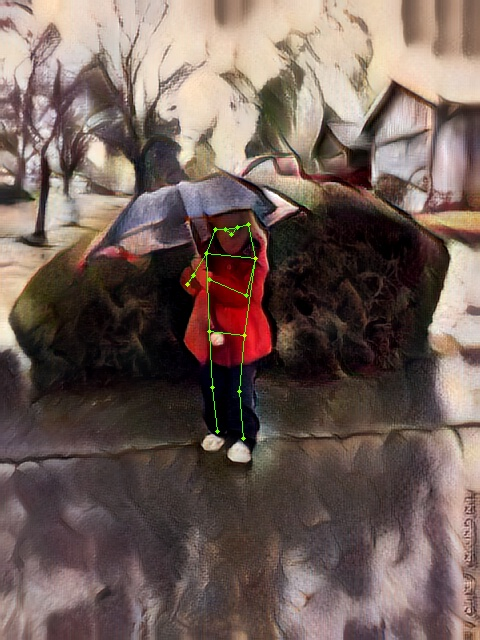
\includegraphics[height=1.75in]{vitpose_7088}
		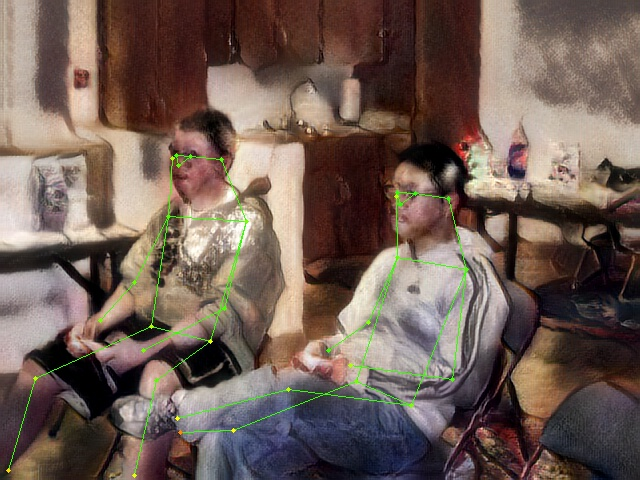
\includegraphics[height=1.75in]{vitpose_91500}
		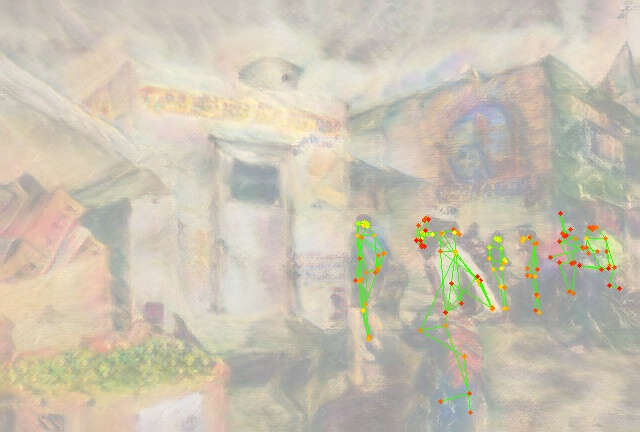
\includegraphics[height=1.75in]{vitpose_259640}
	}
	\caption{
        Examples of the keypoints found by the pre-trained Pose Estimation networks.
    }
    \label{fig:baseline_pose_estimation_evalutaion}
\end{figure}

\begin{table}[h]
    \setlength\tabcolsep{4pt}
    \caption{
        Establishing a baseline for Pose Estimation on Artworks; measuring Average Precision/Recall (AP/AR).
        The COCO dataset is transformed with various Style Transfer models on which performance is measured from pre-trained pose-estimation models. }
    \centering
    \footnotesize
    \label{tab:baseline_pose_estimation_after_style_transfer}
    \begin{tabular}{ l|ccccc|ccccc }
        \hline
        \bf{Method}&\bf{AP}&\bf{AP$^{50}$}&\bf{AP$^{75}$}&\bf{AP$^{M}$}&\bf{AP$^{L}$}&\bf{AR}&\bf{AR$^{50}$}&\bf{AR$^{75}$}&\bf{AR$^{M}$}&\bf{AR$^{L}$}\cr
        \hline
        \multicolumn{11}{c}{\bf{AdaIN}}\cr
        \hline
        SWAHR & 0 & 0 & 0 & 0 & 0 & 0 & 0 & 0 & 0 & 0 \cr
        ViTPose & 0.026 & 0.057 & 0.020 & 0.017 & 0.041 & 0.340 & 0.568 & 0.337 & 0.187 & 0.539 \cr
        \hline
        \multicolumn{11}{c}{\bf{CycleGAN}}\cr
        \hline
        SWAHR & 0 & 0 & 0 & 0 & 0 & 0 & 0 & 0 & 0 & 0 \cr
        ViTPose & 0.081 & 0.128 & 0.086 & 0.120 & 0.068 & 0.627 & 0.850 & 0.682 & 0.557 & 0.718 \cr
        \hline
    \end{tabular}
\end{table}

\section{Pose Estimation on the Human-Art Dataset}
\label{sec:baseline_human_art}
As a second baseline, the Human-Art dataset contains a subset of annotated oil paintings compatible with the COCO format.
The evaluation dataset contains 250 images with 900 annotated persons.
This will give a insight in the performance of the pose estimation models on artworks.
SWAHR and ViTPose will be validated, and the trained weights mentioned in section \ref{sec:baseline_training_pose_estimation} as well as the pre-trained weights from the original papers will be used.
The input image will not be resized or otherwise distorted, and the default parameters used.
To confirm the premise that the pose estimation models perform less well on artworks, they are also validated on the COCO dataset.
Because the other tests are only done on a subset of the COCO dataset, the models are also validated on this subset.
This is a total of 8 combinations that will be validated.

\subsection{Results}
\label{sec:baseline_human_art_results}
As mentioned in section \ref{sec:baseline_results_coco_style_transfer}, only the Average Precision/Recall will be measured.
The table \ref{tab:baseline_pose_estimation_after_style_transfer} shows the results of the measurements.
It clearly shows that the models have inferior results on artworks than photographs by up to 20\%.
It also shows a significant difference between the pre-trained and self-trained models.
However, for SWAHR the pre-trained model performed better by 6\%, but for ViTPose, the self-trained model performs better by 2\%.
This difference well justifies the training of the models on the plain COCO dataset instead of using the pre-trained models to compare to.
Thus going forward, the metrics will be compared to the self-trained models.
This will give a more accurate picture of the improvements made.
Notable as well is that despite ViTPose being the state-of-the-art, it performs worse than SWAHR on both datasets.

\begin{table*}
    \setlength\tabcolsep{4pt}
    \vspace{0.2em}
    \caption{
        Establishing a baseline for Pose Estimation on Artworks; Average Precision/Recall (AP/AR).
        The table shows the performance of the pre-trained models measured on The COCO dataset and the Human-Art dataset.
    }
    \centering
    \footnotesize
    \label{tab:baseline_pose_estimation_after_style_transfer}
    \begin{tabular}{ l|ccccc|ccccc }
        \hline
        \bf{Method}&\bf{AP}&\bf{AP$^{50}$}&\bf{AP$^{75}$}&\bf{AP$^{M}$}&\bf{AP$^{L}$}&\bf{AR}&\bf{AR$^{50}$}&\bf{AR$^{75}$}&\bf{AR$^{M}$}&\bf{AR$^{L}$}\cr
        \hline
        \multicolumn{11}{c}{\bf{COCO dataset}}\cr
        \hline
        Pre-trained SWAHR & \textbf{0.687} & \textbf{0.881} & \textbf{0.748} & \textbf{0.639} & \textbf{0.757} & 0.737 & 0.904 & 0.788 & 0.670 & \textbf{0.828} \cr
        SWAHR & 0.620 & 0.830 & 0.684 & 0.604 & 0.653 & 0.710 & 0.891 & 0.765 & 0.640 & 0.803 \cr
        Pre-trained ViTPose & 0.588 & 0.832 & 0.641 & 0.573 & 0.629 & 0.723 & 0.906 & 0.782 & 0.682 & 0.786 \cr
        ViTPose & 0.609 & 0.847 & 0.680 & 0.597 & 0.644 & \textbf{0.740} & \textbf{0.918} & \textbf{0.810} & \textbf{0.703} & 0.795 \cr
        \hline
        \multicolumn{11}{c}{\bf{Human-Art Dataset}}\cr
        \hline
        Pre-trained SWAHR & \textbf{0.528} & \textbf{0.759} & \textbf{0.565} & 0.099 & \textbf{0.573} & \textbf{0.593} & 0.635 & 0.629 & 0.177 & \textbf{0.635} \cr
        SWAHR & 0.492 & 0.742 & 0.536 & 0.058 & 0.539 & 0.563 & 0.784 & 0.606 & 0.109 & 0.605 \cr
        Pre-trained ViTPose & 0.380 & 0.656 & 0.385 & 0.108 & 0.420 & 0.571 & 0.803 & 0.620 & 0.279 & 0.599 \cr
        ViTPose & 0.406 & 0.682 & 0.415 & \textbf{0.130} & 0.445 & 0.591 & \textbf{0.818} & \textbf{0.632} & \textbf{0.306} & 0.619 \cr
        \hline
        \multicolumn{11}{c}{\bf{Difference}}\cr
        \hline
        Pre-trained SWAHR & -0.159 & -0.122 & -0.183 & -0.540 & -0.184 & \textbf{-0.144} & -0.269 & \textbf{-0.159} & -0.493 & -0.193 \cr
        SWAHR & \textbf{-0.128} & \textbf{-0.088} & \textbf{-0.148} & -0.546 & \textbf{-0.114} & -0.147 & -0.107 & -0.159 & -0.531 & -0.198 \cr
        Pre-trained ViTPose & -0.208 & -0.176 & -0.256 & \textbf{-0.465} & -0.209 & -0.152 & -0.103 & -0.162 & -0.403 & -0.187 \cr
        ViTPose & -0.203 & -0.165 & -0.265 & -0.467 & -0.199 & -0.149 & \textbf{-0.100} & -0.178 & \textbf{-0.397} & \textbf{-0.176} \cr
        \hline
    \end{tabular}
\end{table*}

\section{Discussion}
\label{sec:baseline_human_art_discussion}
The results show that the use of style transfer on the input image will not yield any good results.
The models don't perform well on the stylized images, likely because they don't produce high-fidelity transformations.
Putting a second algorithm in the pipeline creates an extra chance for error.
However, ViTPose was still able to discern most of the poses; having a high recall, but seems to have hallucinated others; giving a low precision.
Which begs the question: What about this network makes it perform better than SWAHR here?
Perhaps, it is merely able to deal with the artifacts left by the style transfer better, while SWAHR is completely confused by it?
Figure \ref{fig:baseline_style_transfer_artifacts} shows these artifacts.
Or, perhaps, it is merely because as a top-down algorithm, it has an unfair advantage in that it used the ground-truth bounding boxes to crop the image.

The baseline on the plain COCO dataset confirms once more that the pose estimation models are inferior on artworks than photographs.
It goes up as high as 50\% for the medium areas, which makes sense as the smaller parts of an image will also be more abstract as brush strokes become more prominent.

\begin{figure}
    \centering
	\subcaptionbox{AdaIN with impressionism as style.}[\textwidth]{
		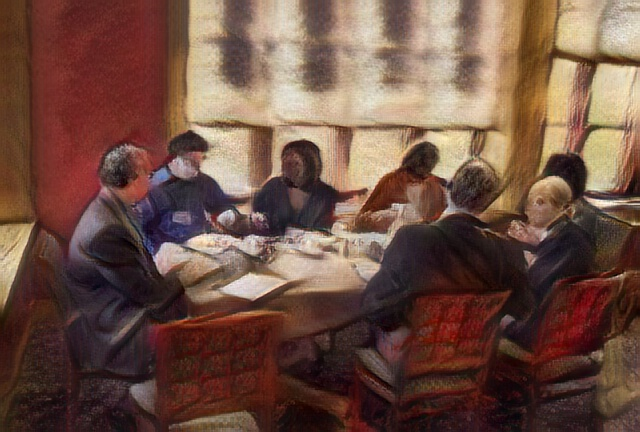
\includegraphics[height=1.75in]{adain_style_transfer_151820}
		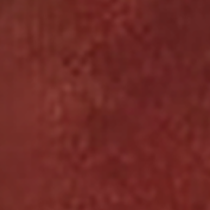
\includegraphics[height=1.75in]{adain_style_transfer_151820_patch_a}
		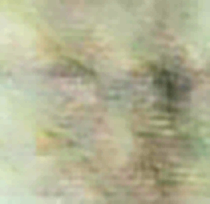
\includegraphics[height=1.75in]{adain_style_transfer_151820_patch_b}
    }
    \subcaptionbox{CycleGAN using impressionism as style}[\textwidth]{
		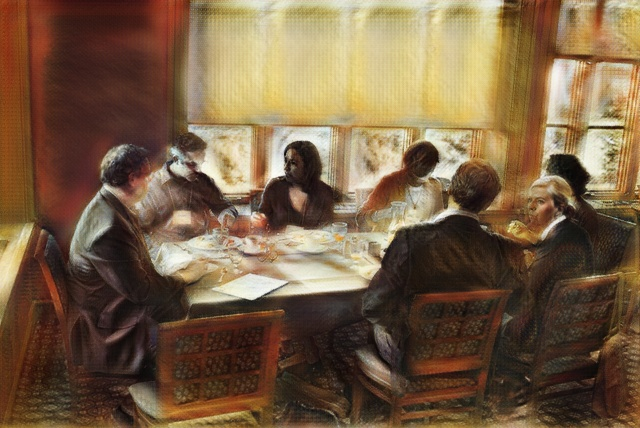
\includegraphics[height=1.75in]{cyclegan_style_transfer_151820}
		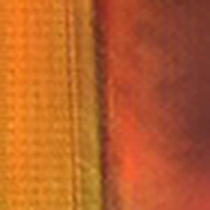
\includegraphics[height=1.75in]{cyclegan_style_transfer_151820_patch_a}
		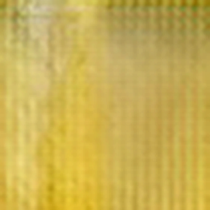
\includegraphics[height=1.75in]{cyclegan_style_transfer_151820_patch_b}
	}
	\caption{
        Examples of artifacts left by AdaIN and CycleGAN. The left images are stylized images, and the right images are close-ups of different patches.
    }
    \label{fig:baseline_style_transfer_artifacts}
\end{figure}